\documentclass[../template]{subfiles}

\newcommand{\idiff}{\ensuremath{I = \frac{dQ}{dt}}}

\begin{document}
\section{Dispositivi e Circuiti Elettronici}
La corrente elettrica $\idiff$ è generata da movimenti di carica. Uno tra i diversi in moto per spostare delle cariche è attraverso un campo elettrico.

La densità di corrente elettrica $J$ è legata al campo elettrico $E$ dalla conducibilità elettrica $\sigma$ attraverso la legge di ohm $\bar{J} = \sigma \bar{E}$.
I materiali sono classificabili dal loro valore di $\sigma$, i materiali isolanti sono caratterizzati da bassi valori di $\sigma$, corrispondenti a bassi valori di corrente.
Valori di $\sigma$ alti comportano un'alta corrente, caratteristica dei materiali conduttori.

I semiconduttori sono materiali con conducibilità elettrica $\sigma$ variabile (ad esempio in funzione della temperatura).
Guardando il caso del componente resistenza, la corrente ai capi di essa dipende dall'inverso della costante $R$, quindi, a tensione costante, maggiore è la resistenza, minore è la corrente misurata ai due capi del componente.

\begin{figure}[h]
    \centering
    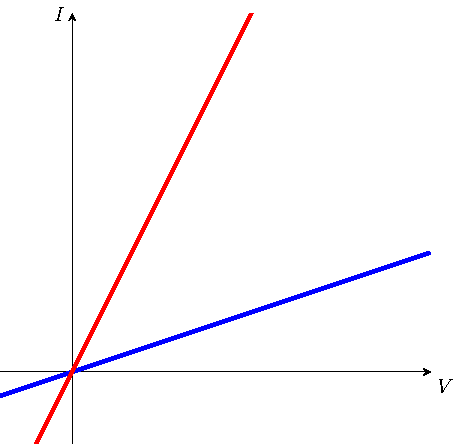
\includegraphics[width=.30\textwidth]{img/resistence-current}
    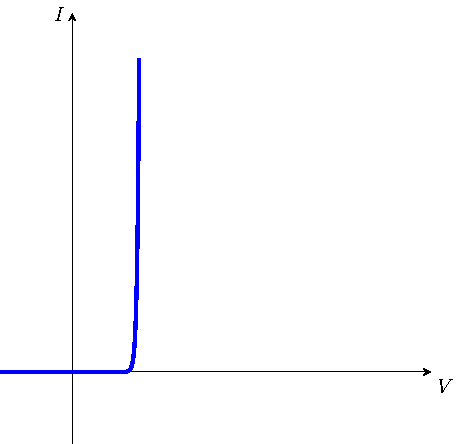
\includegraphics[width=.30\textwidth]{img/diode-current-graph}
\end{figure}
In figura sono riportate le relazioni corrente-tensione di una resistenza ed un diodo. È possibile osservare come il comportamento della corrente del diodo è completamente differente.

\subsubsection{Modello fisico}
Gli elettroni di ciascun materiale orbitano attorno ai rispettivi nuclei, in stato di equilibrio.
In stato equilibrio, gli elettroni di un materiale orbitano attorno al nucleo, la complessiva somma delle cariche risulta nulla.

Gli elettroni attratti dalla forza coulombiana, orbitano attorno al nucleo. Ad ogni orbita corrisponde una velocità di percorrenza,
quindi un'energia cinetica. L'ampiezza di ogni orbita dipende inversamente dal quadrato della distanza dal nucleo (formula forza di coulomb).
\\
In definitiva, possiamo

% TODO

Maggiore è la grandezza dell'orbita degli elettroni, maggiore è la veloci
Inoltre maggiore è la grandezza dell'orbita degli elettroni, maggiore è la velocità degli elettroni, quindi la loro energia cinetica.

All'ampiezza dell'orbita è quindi associato inversamente la forza attrattiva del nucleo, ed un'energia cinetica legata alla velocità di percorrenza.
\\
Possiamo quindi, gli elettroni interni ad un atomo generico in funzione dell'energia da essi posseduta, ottenendo un diagramma simile a quello in figura ..., distinta da diversi livelli

\begin{figure}[h]
    \centering
    \begin{tikzpicture}
        \draw[->] (0, 0) -- (0, 3)
            node[right]{$E$};

        \foreach \y in {.5, 1, ..., 2.5}
        {
            \draw (-3pt, \y) -- (+3pt, \y);
        }
    \end{tikzpicture}
\end{figure}

Ad ogni elettrone è dunque associato un livello sull'asse delle energie.
Per il principio di quantizzazione, dell'energia, non tutti i possibili livelli di energia sono possibili. L'asse quindi non è continua, ma quantizzata.

È importante notare che le orbite degli elettroni attorno agli atomi non sono descritte dalla meccanica classica, ma dalla meccanica quantistica, dove gli elettroni sono descritti attraverso forme sinusoidali.

Per questo motivo è possibile associare agli elettroni una lunghezza d'onda $\lambda$, dove nel caso di ipotesi stazionaria, è necessario che la circonferenza dell'orbita sia multiplo di $\lambda$.
\\
Questo spiega a grandi linee la presenza di valori permessi e proibiti sull'asse delle energie.

\subsubsection{Principio di esclusione di Pauli}
Ciascun livello energetico è occupabile al più da due elettroni (con spin opposto). In altre parole, il numero di elettroni che possono avere una certa distanza dal nucleo è finito.

Da questo è possibile dedurre che è possibile occupare interamente i livelli di energia.

Spostare corrente vuol dire spostare elettroni, cambiandone la velocità, quindi aumentandone l'energia cinetica, vincolata dai livelli di energia e dal principio di esclusione.

Per muovere un'elettrone quindi serve almeno l'energia per raggiungere il livello energetico libero più vicino.

Nel momento in cui due atomi diventino abbastanza vicini da interagire, quello che mi posso aspettare è che gli elettroni dei rispettivi atomi esercitino una forza repulsiva, con l'effetto di modificare l'orbita dei due elettroni.

Considerando quindi un unico diagramma energetico per il sistema dei due atomi, quello che ottengo è che i livelli non si sovrappongono ma si scostano leggermente, mantenendo comunque i principi di quantizzazione ed esclusione.

Generalizzando il discorso con un'interazione di $n$ atomi, otteniamo che ai precedenti livelli energetici, corrisponderà una moltitudine di livelli permessi, tra loro poco differenti, chiamata \textit{banda permessa}.
\\
I valori di energia tra due bande permesse, prendono il nome di \textit{banda proibita}.

È importante sottolineare che i valori interni alla banda permessa rispettano ancora il principio di esclusione e di quantizzazione, quindi è possibile che un'intera banda sia occupata da elettroni.

In condizione di quiete, gli elettroni tendono spontaneamente ad occupare i livelli con minore energia, quindi quelli più bassi.

La statistica di fermi indica un valore limite (\textit{Livello di Fermi}) che indica, in assenza di perturbazione, in termini probabilistici, tutti i livelli che sotto tale valore risultano occupati.

La posizione di questo livello diventa quindi fondamentale per indicare le condizioni di trasporto di carica del materiale.
Nel caso di materiali conduttori, il livello di fermi ricade internamente ad una banda permessa,
l'energia richiesta per spostare elettroni da livelli energetici occupati a livelli energetici liberi, è dipendente dalla loro distanza, quindi molto bassa.

Nel caso di materiali isolanti, il livello di fermi ricade all'interno di una banda proibita, l'energia sufficiente richiesta (energy gap) è quella per scavalcare l'intera banda proibita, quindi molto superiore al caso precedente.

I materiali isolanti sono dunque anch'essi soggetti a fenomeni di scarica elettrica.

\subsubsection{I semiconduttori}
Il semiconduttore ha una struttura simile a quella dell'isolante, quello che differisce è l'ampiezza del gap, richiedendo una quantità di energia bassa per effettuare il "salto" della banda proibita.
Se la quantità di energia ricevibile dalla temperatura dall'ambiente è pari o superiore al gap, diventa facile che elettroni passino da una banda energetica superiore.
Elettroni quindi nella banda permessa superiore, trovandola completamente vuota, richiedono a loro volta poca energia per muoversi da un livello energetico all'altro, fornendo al materiale caratteristiche di un conduttore.
Chiameremo quindi questa nuova banda, banda di conduzione, mentre chiameremo la vecchia banda, banda di valenza.

La banda di valenza, avendo anch'essa livelli svuotati da elettroni spostati in banda di conduzione, richiederà anch'essa poca energia per effettuare salti di gap interni alla banda.
La conducibilità elettrica aumenta quindi con la temperatura del circuito.

Riassumendo quindi, un semiconduttore il livello di fermi interseca una banda proibita, la cui ampiezza è sufficientemente piccola da essere probabile l'effetto di scavalcamento con la sola energia termica.
Il semiconduttore ha quindi "due" bande di conduzione.


% seconda lezione
\subsubsection{Seconda lezione}
la distanza dal nucleo cresce col crescere dell'energia, andando a vedere gli elettroni sullo strato di valenza, sono quelli più distanti dal nucleo.
La forma del reticolo di atomi è determinata dal numero di elettroni disponibili a collegarsi agli atomi vicini.
Tutti i materiali semiconduttori sono materiali della quarta colonna della tavola periodica, i quali possiedono quattro elementi nell'orbita di legame, tra essi prevale il silicio.

In alternativa agli elementi della tavola periodica è possibile formare delle leghe tra elementi della terza e quarta colonna o quarta e quinta, come arseniuro di gallio.

Schematizzando il reticolo del silicio su una mappa in due dimensioni (figura ?)
La promozione da banda di valenza a banda di conduzione, significa che esso è meno legato al nucleo originario. È talmente poco legato al nucleo che attraverso una forza di un campo magnetico può spostarsi internamente al reticolo.
Tali elettroni vengono definiti come elettroni liberi.

Il materiale in condizione di quiete è neutro, ovvero ha tanta carica positiva quanta negativa. Al momento in cui un'elettrone libero esce da una regione, quella regione non ha più carica nulla ma leggermente positiva. Possiamo quindi immaginare il moto dell'elettrone come uno spostamento di carica nello spazio, quindi una corrente.
\\
Lo spazio lasciato vuoto dall'elettrone, è successivamente occupato da altri elettroni liberi. Creando uno spostamento a catena degli elettroni.

Alla banda di conduzione è associato il movimento di una carica negativa, alla banda di valenza è associato il movimento della lacuna, carica positiva generata dallo spostamento dell'elettrone.

In un conduttore esiste solo un tipo di portatore di carica (elettroni), mentre nei semiconduttori esistono portatori di carica positiva e portatori di carica negativa.

È possibile modellare il movimento della lacuna come il movimento di una fittizia particella fisica, dotata di una massa (maggiore di quella dell'elettrone perché si muove più lentamente)

Per misurare la corrente è necessario conoscere la quantità di elettroni e lacune in un determinato volume.
Indicheremo quindi con $n$ il numero di elettroni per unità di volume \footnote{Misurata per numero di elettroni per centimetro cubo}.
Analogamente definiamo la concentrazione di lacune con $p$ come il numero di lacune per unità di volume.

Per densità di carica degli elettroni si calcola con $-qn$, mentre per lacune $qn$.
Ad ogni elettrone libero in banda di valenza, corrisponde una lacuna in banda di conduzione, quindi necessariamente all'equilibrio $p = n$.

Possiamo quindi definire come evento di generazione il momento in cui un'elettrone abbandona la banda di valenza generando una lacuna, mentre il fenomeno duale, il passaggio da banda di conduzione a bassa di valenza viene chiamato evento di ricombinazione.

Indichiamo quindi con $G$ il numero di coppie elettrone-lacune generate nell'unità di volume e nell'unità di tempo. Il tasso di ricombinazione è indicato con $R$.

Alla equilibrio quindi $n = p = n_i(T)$ e $R = G\ge 0$ il numero di elettroni e lacune costante prende il nome di $n_i$ (concentrazione intrinseca del materiale).

Sostituendo ad alcuni atomi di silicio, con atomi della 5a colonna, as es fosforo. In questo modo avendo un'elettrone di legame in più (ed un protone in più), siccome i legami sono tutti occupati con gli atomi di silicio adiacenti, otteniamo un'elettrone che non contribuisce ad alcun legame nel reticolo.
\\
La sostituzione di alcuni atomi di silicio con atomi della 3a o 5a colonna prende il nome di drogaggio.

La rara sostituzione di atomi di silicio, non varia il reticolo cristallino originario.

L'elettrone nella fascia più esterna non essendo legato agli altri se riceve energia sufficiente può liberarsi e comportarsi come una carica negativa mobile. È ancora vero che lascia alle sue spalle una carenza di carica negativa, ma la carica positiva è associata alla presenza del protone nel nucleo e non è in grado di spostarsi.
In questo caso si genera un'elettrone mobile, senza generare lacune mobili. In questo caso $p \neq n$. Gli atomi della quinta colonna prendono quindi il nome di atomi droganti di tipo donatore.

Tutto questo è rappresentabile nel diagramma delle energie inserendo un livello "donatore" interno alla banda proibita permettendo che l'evento di liberazione dell'elettrone richieda meno energia, rendendolo ancora più probabile a temperatura ambiente.
\\
Chiameremo $N_D$ la concentrazione di atomi donatori, e per mantenere la struttura del cristallino $N_D \ll 10^{22}$.

Analogamente prendendo un' elemento della terza colonna (es. boro) nel reticolo viene rimosso un legame, fornendo energia al reticolo e spostando elettroni, essi andranno ad occupare del legame mancante, generando lo spostamento di una carica positiva.
La carica negativa è fissa perché legata alla struttura del boro.

Chiameremo il boro atomo accettore, perché capace di ionizzare il reticolo negativamente. Con $N_A$ indicheremo la concentrazione degli atomi accettori per unità di volume. Interpretando l'evento sul diagramma energetico, sarebbe come un livello energetico che ricade nella banda proibita molto vicino alla banda di valenza. Generando una lacuna mobile in tale banda.

In questo caso $n < p$.

\subsubsection{Terza Lezione}
Abbiamo interpretato il diverso comportamento delle due bande, elettroni liberi che si muovono tra livelli energetici nella banda di conduzione, e lacune alle quali è associato un significato di carica positiva mobile.
\\
In un materiale intrinseco, elettroni e lacune sono creati sempre in coppia, quindi necessariamente la concentrazione di elettroni e lacune sono uguali alla concentrazione intrinseca, dipendente dalla temperatura.

Inoltre in condizioni di equilibrio il tasso di generazione $G$ e di ricombinazione $R$ devono essere uguali.

L'equivalenza tra elettroni e lacune interna al materiale può essere modificata attraverso drogaggi con atomi donatori ($N_D$) o accettori ($N_A$). La concentrazione elettroni-lacune in materiali drogati è chiamata concentrazione estrinseca.

Supponendo di conoscere la concentrazione tra atomi donatori ed accettori, calcoliamo ora i nuovi valori di $p$ ed $n$ interni al materiale.

Osservando il caso della concentrazione intrinseca, osserviamo che necessariamente il prodotto $pn = n_i^2$. Questa relazione è valida non solo per materiali intrinseci, ma anche per materiali estrinseci.

Possiamo pensare che il tasso di generazione $G$ sia dipendente unicamente dalla temperatura: $g(T)$. Mentre il tasso di ricombinazione $R$, l'occupazione di una lacuna da parte di un'elettrone, è logico pensare che dipenda dal numero di elettroni presenti nel materiale e dalla temperatura: $R = pnr(T)$.
\\
Il tasso di generazione non dipende dalla concentrazione effettiva di $p$ ed $n$, perché per evitare che si effettui una generazione, tutti gli elettroni in banda di valenza dovrebbero essersi spostati in banda di conduzione. Ipotesi irragionevole a temperatura ambiente.

Ricordandoci che in condizioni di equilibrio $G = R$, otteniamo che $g(T) = pnr(T)$. Quindi $pn = g(T)/r(T) = f(T)$ è dipendente unicamente dalla temperatura. Quindi a temperatura costante il valore $pn$ è costante e vale $n_i^2$.

Inoltre se è vero che a livello globale la quantità di carica positiva equivale alla carica negativa, allora la densità di carica $\rho$ in tutto il volume è costante e pari a $0$.

\[
    \rho = -q n + qp  + qN_D -q N_A = q (p -n + N_D - N_A) = 0
\]
La densità di carica dipende dal numero di elettroni $n$ e lacune $p$ con rispettiva carica, ed il numero di atomi accettori e donatori interni ad un materiale, ad ognuno dei quali è associata rispettivamente una carica fissa in modulo $q$.
\\
Unendo la relazione con $pn = n_i$, ricaviamo:
\[
    n = \frac{(N_D - N_A) \pm \sqrt{(N_D - N_A)^2 + 4 n_i^2}}{2}
\]
Siccome è evidente che non può valere il segno meno in quanto condurrebbe ad un valore di $n$ negativo, ottengo un'espressione del valore di $n$ dipendente solo da valori noti.
\\
Con questo ragionamento otteniamo anche il valore di $p$:
\[
    p = \frac{(N_A - N_D) + \sqrt{(N_A - N_D)^2 + 4 n_i^2}}{2}
\]

Dalle espressioni si può osservare come compare sempre la differenza dei valori $N_D$ ed $N_A$, il fenomeno prende il nome di principio di compensazione, il quale dice che non è importante il singolo valore di $N_D$ ed $N_A$, quello che conta è sempre la loro differenza.


Nel caso di una concentrazione con forte sbilanciamento, es $N_D \gg N_A \gg n_i$, nelle equazioni in precedenza, posso trascurare i termini $N_A$ ed $n_i$, ottenendo $n = N_D$.
Quindi se la concentrazione del drogante è molto maggiore rispetto alla concentrazione intrinseca, allora la concentrazione di elettroni è dovuta praticamente solo ad esso.
Siccome vale $pn = n_i^2$, abbiamo che $p = n_i^2 / N_D$. Segue che il trasporto della carica, avviene quasi unicamente attraverso elettroni.
\\
Chiameremo questo materiale "estrinseco di tipo n", ad indicare la larga prevalenza degli elettroni.

Posso effettuare gli stessi ragionamenti nel caso duale ($N_A \gg N_D \gg n_i$), ottenendo $p = N_A$ e $n = n_i^2 / N_A$.
Chiameremo questo materiale "estrinseco di tipo p".

\subsubsection{Studio conduzione materiale uniforme, estrinseco di tipo n}

Conoscendo la conduzione del materiale $n \approx N_D$, ed indicando con $S$ la sezione trasversale del materiale, indicheremo $J = I/S$.
Ricordando che $I = dQ/dt$, otteniamo:
\[
    J = \frac{1}{S}\frac{dQ}{dt}
\]
Sapendo che il calcolo elettrico $E$ esercita una forza di coulomb pari a $F = -qE$, ed $F = ma$, otteniamo $a = -qE/m$, quindi accelerazione costante a campo elettrico costante. Quindi un'elettrone dovrebbe muoversi di moto uniformemente accelerato.
\\
Ma ciò non è vero perché l'elettrone è soggetto anche alle forze interne al reticolo cristallino. Quindi è soggetto ad una forza repulsiva . Quello che si può vedere sperimentalmente è che la velocità $V_n$ è costante ed esprimibile come $V_n = -\mu_n E$, con $\mu_n$ costante di mobilità elettronica.

Gli elettroni si muovono quindi in direzione opposta al campo elettrico, con velocità $|V_n|$.
Il percorso che percorre una singola particella in un piccolo intervallo di tempo è esprimibile quindi come $dx = -\mu_n E dt$.
\\
La carica $dQ$ è quella che nello stesso intervallo di tempo $dt$ attraversa la sezione del materiale, è possibile pensarla come $nq S dx$ (carica del numero di portatori nel volume $Sdx$).

Quindi la densità $J$ è esprimibile come:
\[
    J_n = \frac{1}{\cancel{S}} \frac{qn\cancel{S} \mu_n E \cancel{dt}}{\cancel{dt}} = qn\mu_n E
\]
Vale ancora la relazione di ohm in forma locale $J = \sigma E$, con $\sigma = qn \mu_n = q \mu_n N_D$.
È possibile concludere che $N_D$ è direttamente proporzionale alla conducibilità elettrica. Quindi possiamo variando dinamicamente il valore di $N_D$ si può ottenere un conduttore o un isolante.

Quindi solo variando il valore di $N_D$ in una parte del materiale posso formare due regioni conduttive, separate da una isolante.

\subsubsection{Conduzione materiali estrinseci di tipo p}
Con ragionamento del tutto analogo al precedente, si ottiene che la velocità di mobilità delle lacune è pari a $V_p = \mu_p E$.
Nel dettaglio $\mu_p \approx \frac{2}{3} \mu_n$, sottolineando che le lacune si comportano come particelle fittizzie che si muovono più lentamente degli elettroni.

Ottenendo
\[
    J_p = \frac{1}{S}\frac{qp\mu_pESdx}{dt} = qp\mu_p E
\]
In questo caso la conducibilità elettrica è determinata da $N_A$.

La totale conducibilità elettrica è possibile esprimerla come $J = J_n + J_p$. $J$ conta la quantità di carica che attraversa la sezione, quindi gli elettroni portano contributo positivo muovendo carica negativa in senso opposto, e le lacune portano contributo positivo.
\[
    J = J_n + J_p = qn\mu_n E + qp \mu_p E
\]
\subsubsection{Materiale drogato non uniformemente}

Nel caso in cui il campo elettrico esterno sia nullo, gli elettroni si spostano ugualmente per il moto browniano.
Possiamo pensare alla carica $dQ$ come $dQ_1 - dQ_2$ ovvero la carica dovuta agli elettroni che escono dalla sezione di volume, e la carica degli elettroni entranti nella sezione di volume.
Chiamata quindi $n_1$ la quantità di elettroni presente nel primo volume, e $n_2$ la quantità di elettroni nel secondo; siccome le cariche hanno un 50\% di probabilità di entrare nel volume, si possono esprimere le cariche come:
\begin{align*}
    dQ_1 = -\frac{q n_1 dV}{2}\\
    dQ_2 = -\frac{q n_2 dV}{2}
\end{align*}
Ricordando che il volume $dV = S V_{th} dt$ si ottiene che:
\[
    J_n = \frac{1}{S} \frac{-qn_1 S V_{th} dt + qn_2 S V_{th} dt}{2dt}  = q(n_2 - n_1) V_{th} \neq 0
\]
Ma siamo giunti ad un assurdo, in quanto avremmo trovato un modo per generare corrente senza spendere energia.

Effettuando i calcoli più accuratamente è possibile ottenere $J_n = q D_n \frac{dn}{dx}$. Quello che accade è il fenomeno della diffusione, infatti tende a muovere la carica, dalla regione di concentrazione più alta a quella più bassa. Il sistema evolve verso una distribuzione uniforme.
\\
Lo spostamento degli elettroni lascia cariche positive nella regione con maggior carica negativa, portando una carica negativa nell'altra regione.

Otteniamo quindi un campo elettrico nella direzione della regione con meno cariche negative, pari a $F = -qE$.

\subsection{Lezione 4}
% 17.03
Analogamente al caso precedente, studiamo un materiale estrinseco di tipo p, la cui concentrazione di lacune non è costante, ottenendo:
\[
    J_p = \frac{1}{S}\frac{d(Q_1 - Q_2)}{dt} = \frac{q(p_1 - p_2) V_{th}}{2}
\]
contrariamente al caso degli elettroni, se $p_2 > p_1$ otteniamo $J_p < 0$.
In questo, effettuando i calcoli in maniera più accurata, otterremo che $J_p = -qD_p \frac{dp}{dx}$.

Abbiamo introdotto quindi i funzionamenti di tipo ohmico: $J_n = q\mu_n n E$ e $J_p = q \mu_p p E$, la cui direzione è concorde;
ed un meccanismo di tipo diffusivo: $J_n = q D_n \frac{dn}{dx}$ e $J_p = -qD_p \frac{dp}{dx}$, la discordanza di segno è dovuta al bilanciamento della carica.

Non possiamo considerare i due funzionamenti come uno indipendente dall'altro, in quanto porterebbe a conclusioni assurde, esprimiamo quindi la combinazione degli effetti:
\begin{align*}
    J_n = q \mu_n n E + q D_n \frac{dn}{dx} \\
    J_p = q \mu_p p E + q D_p \frac{dp}{dx}
\end{align*}

Quindi un conduttore prevede un solo meccanismo di trasporto di carica, per un meccanismo unicamente di tipo ohmico. In un semiconduttore teniamo conto di due specie di carica e di due specie di carica e due diversi meccanismi di trasporto di carica: trasporto ohmico e diffusivo.

Il modello prende infatti il nome di ohmico-diffusivo (\textit{drift-diffusion}).

$D_n$ indica la reattività dell'elettrone alla temperatura.
\[
    D_n = \frac{kT}{q} \mu_n
\]
Analogamente $D_p = \frac{kT}{q}\mu_p$. Queste prendono il nome di relazioni di Einstein, dove $k$ è la costante di Boltzmann, $q$ è la carica dell'elettrone e $T$ è la temperatura.

Quello che dicono queste relazioni è che il coefficiente di diffusione e la mobilità dell'elettrone, sono legate.
Ricordando che la mobilità degli elettroni è superiore a quella delle lacune, analogamente il fattore $D_n$ è maggiore di $D_p$
% 37:50

Ricordandoci che $E = -\frac{d\phi}{dx}$
prendiamo in considerazione, un materiale, tale per cui la concentrazione varia in base alla coordinata $x$: $n(x)$.
Siccome il campo elettrico $E$, costante ed indipendente dalla posizione $x$, prendiamo un punto $x_1$ interno al materiale e lo usiamo come origine per misurare il campo elettrico. In tale punto avremo che $\varphi = 0$, $n_0$ e $p_0$.

Allo stesso identico modo posso scegliere un punto $x_2$, caratterizzato da un $\varphi(x)$, $n(x)$ e $p(x)$.

All'equilibrio $pn = n_i^2$, otteniamo che, dalla funzione di $J_n = q \mu_n  n E + q D_n \frac{dn}{dx} \approx 0$, otteniamo:
\[
    \frac{kT}{nq} \frac{dn}{dx} = \frac{d\varphi}{dx}
\]

Integrando la relazione sui margini $\varphi(0)$ e $\varphi(x)$, ottengo:
\[
    \varphi(x) = \frac{kT}{q} \ln \frac{n(x)}{n_0}
\]
Da cui
\[
    n(x) = n_0 e^{\dfrac{q\varphi(x)}{kT}}
\]
Inoltre dalla relazione $p(x) n(x) = n_i^2$, otteniamo la relazione duale $p(x) = p_0 e^{-q\varphi(x) / kT}$ la inversa $\varphi(x) = - \frac{kT}{q} \ln \frac{p(x)}{p_0}$.

% maxwell
Dalle equazioni di Maxwell, per i materiali uniformi: $\frac{d^2 \varphi}{dx} = -\frac{\rho}{\varepsilon}$
\subsection{Ragionamento su struttura diversamente drogata}
Supponiamo un unico cristallo di semiconduttore, drogato per metà in con atomi accettori, e per metà con atomi donatori.
Il materiale prende il nome di giunzione pn.


\subsubsection{Studio della struttura all'equilibrio}

Supponiamo una differente distribuzione di atomi accettori e donatori. Prendendo quindi come origine il punto intermedio tra le due giunzioni, otteniamo:

\begin{figure}[h]
    \centering
    \begin{tikzpicture}
        \begin{axis}[xlabel=$x$, ylabel=$$, ymin=-1, ymax=4]
            \addplot[domain=-5:0, red]{0};
            \addplot[domain=0:5, red]{2};
            \addplot[domain=-5:0, blue]{2.5};
            \addplot[domain=0:5, blue]{0};

            \draw (2, 2) node[red, above]{$N_D$}
                (-2, 2.5) node[blue, above]{$N_A$};
        \end{axis}
    \end{tikzpicture}
\end{figure}

Supponiamo che il dispositivo sia abbastanza lungo, da supportare l'ipotesi che dopo una certa distanza, l'effetto della giunzione risulti trascurabile, in modo che sia possibile esprimere le relazioni dei due estremi indipendentemente.
Quindi, che esistano due coordinate $w_p$ e $w_n$, che oltre a quelle coordinate, le due regioni si comportano come regioni uniformemente drogate di tipo $p$ ed $n$.


\begin{tcolorbox}[title={Zona neutra p}]
    Per $x < -w_p$, la popolazione di portatori maggioritaria sono le lacune, quindi $p = N_A$ e $n = \frac{n_i^2}{N_A}$
    \begin{align*}
        \rho = q (\cancel{N_D} - N_A + p - \cancel{n}) \approx  0\\
        J_p = q \mu_p p E - q D_n \frac{dp}{dx} = 0
    \end{align*}
    Essendo la densità di carica pari a 0, e la variazione di atomi portatori nulla, allora necessariamente $E = 0$

    Siccome $E$ dipende dalla derivata di $\varphi$ rispetto ad $x$ allora $\varphi$ è costante. Prendiamo questo valore, come valore di riferimento, per i successivi $\varphi$, quindi $\varphi = 0$.
\end{tcolorbox}
\begin{tcolorbox}[title={Zona neutra n}]
    Per $x > w_n$, $n = N_D$ e $p = \frac{n_i^2}{N_D}$. Inoltre $\rho = q (N_D - n) \approx 0$.
    \[
        J_n = q \mu_n n E + q D_n \frac{dn}{dx} = 0
    \]
    Per analogo ragionamento $E = 0$ e $\varphi$ è costante, calcolabile attraverso la formula
    \[
        \frac{kT}{q} \ln \frac{n(x)}{n_0} = \frac{kT}{q} \ln \frac{N_D N_A}{n_i^2}
    \]
    Indicheremo questo valore con $\Psi_B$. Siccome i valori di $N_D$ ed $N_A$ sono entrambi molto maggiori di $n_i$, allora $\Psi_B$ è positiva e molto maggiore di 1.
    Inoltre siccome dipende dal logaritmo di $N_D$ ed $N_A$, per variazioni di quest'ultimi è assimilabile ad una costante.
\end{tcolorbox}
\begin{tcolorbox}[title={Regione svuotata}]
    Per $-w_p < x < w_n$, ipotizzando che il potenziale sia monotono in questo intervallo, possiamo presupporre che $0 < \varphi(x) < \Psi_B$.

    Quindi in tutto l'intervallo $\varphi(x) > 0$, da cui moltiplicando per la quantità positiva $\frac{q}{kT}$, otteniamo
    \[
        p_0 e^{-\frac{q\varphi}{kT}} \ll p_0 = N_A
    \]
    Il cui primo termine è $p(x)$.
    Analogamente, da ipotesi di funzione monotona, posso dire che $\varphi(x) < \Psi_B$, e moltiplicandola per la stessa quantità positiva $\frac{q}{kT}$ ottengo:

    \[
    n(x) = n_0 e^{\frac{q\varphi(x)}{kT}} \ll n_0 e^{\frac{q\Psi_B}{kT}} = N_D
    \]

    Da cui i valori di $n$ e $p$ sono rappresentati graficamente da valori prossimi a 0.
\end{tcolorbox}
\begin{tcolorbox}[title={Regione svuotata e regione di carica}]
    Per $-w_p < x < 0$
    La densità di carica non sarà più nulla, ma siccome $p(x) \ll N_A$, $n(x) \ll N_D$, in base all'intervallo in cui mi trovo, per la relazione $\rho = q(N_D - N_A + \cancel{p} - \cancel{n})$, la densità di carica potrà valere $-qN_A$ o $qN_D$.
    Per la relazione di poisson: $\frac{dE}{dx} = -\frac{\rho}{\varepsilon}$. Sostituendo rispettivo valore di $\rho$ ed integrando nei relativi estremi, si ottiene il campo elettrico:
    \[
        E = - \frac{qN_A}{\varepsilon} (x + w_p)
    \]
    Nel caso particolare $E(0^-) = \dfrac{-qN_A w_p}{\varepsilon}$

    Dalla relazione $E = -\frac{d\phi}{dx}$, integrando sugli estremi si ottiene:
    \[
        \varphi(x) = \frac{qN_A}{\varepsilon}\frac{{(x + w_p)}^2}{2}
    \]
    con $\varphi(0^-) = \frac{qN_A}{2\varepsilon}w^2_p$
\end{tcolorbox}
\begin{tcolorbox}[title={}]
    Per $0 < x < w_n$, con analoghi ragionamenti, $\rho = qN_D$
    ed il campo elettrico $E$ e potenziale $\phi$ saranno rispettivamente:
    \begin{align*}
        &E(x) = \frac{qN_D}{\varepsilon} (x - w_n) & E(0^+) = - \frac{qN_D}{\varepsilon} w_n\\
        &\phi(x) = \Psi_B - \frac{qN_D}{2\varepsilon} {(x - w_n)}^2 & \psi(0^+) = \Psi_B - \frac{qN_D}{2\varepsilon} w_n^2
    \end{align*}
\end{tcolorbox}

\begin{figure}[h]
    \centering

    \def\wp{-1.2}
    %\def\wn{2}
    \def\eps{1}
    \def\fb{2}
    \def\wn{sqrt(2*\fb/\eps - \wp*\wp)}

    \begin{tikzpicture}
        \begin{axis}[width=.33\textwidth, xlabel=$x$, ylabel=$$]
            \addplot[domain=\wp:5, red]{0};
            \addplot[domain=-5:\wp, red]{1.6};
            \addplot[domain=-5:\wn, blue]{0};
            \addplot[domain=\wn:5, blue]{1.5};
            \draw
                (\wp-1, 1.6) node[above, red]{$p$}
                (3, 1.6) node[above, blue]{$n$}
                ;
        \end{axis}
    \end{tikzpicture}
    \begin{tikzpicture}
        \begin{axis}[width=.33\textwidth, xlabel=$x$, ylabel=$\rho$]
            \addplot[domain=-5:\wp, blue]{0};
            \addplot[domain=\wp:0, blue]{-1};
            \addplot[domain=0:\wn, blue]{1};
            \addplot[domain=\wn:5, blue]{0};
        \end{axis}
    \end{tikzpicture}
    \begin{tikzpicture}
        \begin{axis}[width=.33\textwidth, xlabel=$x$, ylabel=$E$]
            \addplot[domain=-5:\wp, blue]{0};
            \addplot[domain=\wp:0, blue]{\eps*(- x + \wp)};

            \addplot[domain=0:\wn, blue]{\eps*(x - \wn)};
            \addplot[domain=\wn:5, blue]{0};
        \end{axis}
    \end{tikzpicture}
    \begin{tikzpicture}
        \begin{axis}[width=.33\textwidth, xlabel=$x$, ylabel=$\phi$]
            \addplot[domain=-5:\wp, blue]{0};
            \addplot[domain=\wn:5, blue]{\fb};
            \addplot[domain=\wp:0, blue]{\eps * ((x - \wp)^2)/2};
            \addplot[domain=0:\wn, blue]{\fb - \eps * ((x - \wn) ^2 /2)};
        \end{axis}
    \end{tikzpicture}
\end{figure}

Se è presente una corrente diffusiva, è presente anche una corrente opposta di trascinamento ohmico. La regione $-w_p < x < 0$ è sede di carica negativa fissa, e la controparte $ 0 < x < w_n$ è ricca di atomi droganti, che avendo donato elettroni per effetto di diffusione, portano una regione di carica positiva fissa.

Le cariche fisse positive e negative, rappresentano un dipolo di carica, e generano un campo elettrico rivolto verso la regione p.
Per sostenere tale campo elettrico è necessaria una differenza di potenziale.

La condizione di equilibrio è raggiungibile in due modi: o sia la componente ohmica e diffusiva sono nulle, o opposte.
In particolare lo spostamento di elettroni per diffusione forma un campo elettrico ohmico che all'equilibrio è uguale ed opposto.

$\Phi_B$ prende infatti il nome di potenziale di barriera, perché è necessario a sostenere il campo elettrico necessario a bilanciare la diffusione.
\end{document}
